%----------------------------------------------------------------------------------------
%    PACKAGES AND THEMES
%----------------------------------------------------------------------------------------

\documentclass[aspectratio=169,xcolor=dvipsnames]{beamer}
\usetheme{SimpleDarkBlue}

\usepackage{hyperref}
\usepackage{graphicx} % Allows including images
\usepackage{booktabs} % Allows the use of \toprule, \midrule and \bottomrule in tables
\usepackage{tikz}
\usepackage{minted}
\usepackage[T1]{fontenc}
\usepackage{inconsolata}
\usetikzlibrary{positioning}

\setminted{breaklines=true, breakautoindent=true}

\title{National Institute of Informatics Internship Report}
\subtitle{Relation Extraction via Manual Prompting and Prompt Tuning via Light-weight LLM}

\author{Batuhan Karaca}

\institute
{
    Department of Computer Science \\
    University of Freiburg % Your institution for the title page
}
\date{\today} % Date, can be changed to a custom date

%----------------------------------------------------------------------------------------
%    PRESENTATION SLIDES
%----------------------------------------------------------------------------------------

\begin{document}

\begin{frame}
    % Print the title page as the first slide
    \titlepage
\end{frame}

\begin{frame}{Overview}
    % Throughout your presentation, if you choose to use \section{} and \subsection{} commands, these will automatically be printed on this slide as an overview of your presentation
    \tableofcontents
\end{frame}

\section{Background Research}
\begin{frame}{Background Research}
    \begin{columns}[c]
    \column{.45\textwidth}
    \begin{itemize}
        \item Reading the the Book: Knowledge Graphs \cite{hogan_knowledge_2022}
        \item Reading about LLMs 
        \item The Paper: Unifying Large Language Models and Knowledge Graphs: A Roadmap \cite{pan_unifying_2024}
    \end{itemize}
        \column{.45\textwidth}
        \begin{figure}
        \centering
        
\includegraphics[height=0.5\textheight]{pictures/kgbook.jpg}
        \caption{The Book: Knowledge Graphs}
        \label{fig:kgbook}
    \end{figure}
    \end{columns}
\end{frame}

\section{Task: Relation Extraction via Manual Prompting}

\begin{frame}[fragile]{Problem}
    \begin{columns}[c]
        \column{.45\textwidth}
        \textbf{Sentence} \\
        \begin{minted}[fontsize=\normalsize]{text}
The bond insurers declined to comment on friday, though on thursday, mbia 's chief financial officer, charles e. chaplin, vigorously defended his company at a hearing in congress and said it did not need any help.
        \end{minted} 
        \column{.5\textwidth}
        \textbf{Triples}\\
        \begin{minted}[fontsize=\tiny]{python}
[
    ('MBIA', 'org:top_members/employees', 'Charles E. Chaplin'),
    ...
]            
        \end{minted}
    \end{columns}
\end{frame}

\begin{frame}{Task: Relation Extraction via Manual Prompting}
\begin{figure}[H]
\centering
\begin{tikzpicture}[->, >=stealth, shorten >=1pt, auto, node distance=3cm, thick, main node/.style={circle, draw, font=\Large}]

  % Define nodes
  \node[main node,opacity=0,text opacity=1] (s0) {prompt+sentence};
  \node[main node] (s1) [right=1cm of s0] {\textbf{LLM}};
  \node[main node, opacity=0, text opacity=1] (s2) [right=1cm of s1] {[(head, relation, tail), ...]};

  % Define edges with labels (including new s1->s2 edge)
  \path[->] 
    (s0) edge node {} (s1)
    (s1) edge node {} (s2);
\end{tikzpicture}
\label{fig:llm_graph}
\end{figure}
\end{frame}

\begin{frame}[fragile]{Prompt}
\begin{minted}[fontsize=\normalsize]{text}
List of predicates is [...]. What Subject-Predicate-Object triples are included in the task sentence? Each triple is in the form ('subject', 'predicate', 'object'). 'predicate' must be from the list of predicates only. Only use 'NA' when you cannot find any reasonable predicates. Some reference sentence-triple pairs will be given. For each pair, sentence is given after 'Sentence: ' and the corresponding triples are given in a python list after 'Triple: ' word. Only return the triples in a Python list. The task sentence is the last sentence with no triples.
\end{minted}
\end{frame}

\begin{frame}{Points to Consider}
    \begin{itemize}
        \item Accuracy of ground truth KG
        \item Negative LLM outputs not entailed by the labels
        \item Positive LLM outputs that can be entailed by the labels
        \item Number of parameters
    \end{itemize}
\end{frame}

\begin{frame}{Assumptions}
    \begin{itemize}
        \item CWA (i.e. No negative relations)
        \begin{itemize}
            \item[] Accurate constraints 
        \end{itemize}
        \item No other entailments (i.e. unique relations)
    \end{itemize}
\end{frame}

\begin{frame}[fragile]{Sample Sentence}
\begin{minted}[fontsize=\normalsize]{text}
Directed by david gordon green; written by green, based on the novel by stewart o'nan; director of photography, tim orr; edited by william anderson; music by david wingo and jeff mcilwain; production designer, richard wright; produced by dan lindau, paul miller, lisa muskat and cami taylor; released by warner independent pictures. 
\end{minted}    
\end{frame}

\begin{frame}[fragile]{Without predicates}
\begin{columns}[c]
\column{.45\textwidth}
\textbf{ChatGPT}
\begin{minted}[fontsize=\tiny]{python}
[
    ('david gordon green', 'directed by', None),
    ('green', 'written by', None),
    ('green', 'based on', 'the novel by stewart o\'nan'),
    ('tim orr', 'director of photography', None),
    ('william anderson', 'edited by', None),
    ('david wingo', 'music by', None),
    ('jeff mcilwain', 'music by', None),
    ('richard wright', 'production designer', None),
    ('dan lindau', 'produced by', None),
    ('paul miller', 'produced by', None),
    ('lisa muskat', 'produced by', None),
    ('cami taylor', 'produced by', None),
    ('warner independent pictures', 'released by', None)
]
\end{minted}
\column{.45\textwidth}
\textbf{Phi-3-mini}
\begin{minted}[fontsize=\tiny]{python}
[('David Gordon Green', 'Directed by', 'Directed by David Gordon Green'),
 ('David Gordon Green', 'Written by', 'Written by David Gordon Green'),
 ('David Gordon Green', 'Based on the novel by', 'Based on the novel by Stewart O'Nan'),
 ('Tim Orr', 'Director of Photography', 'Tim Orr'),
 ('William Anderson', 'Editor', 'William Anderson'),
 ('David Wingo', 'Music by', 'David Wingo'),
 ('Jeff McIlwain', 'Music by', 'Jeff McIlwain'),
 ('Richard Wright', 'Production Designer', 'Richard Wright'),
 ('Dan Lindau', 'Produced by', 'Dan Lindau'),
 ('Paul Miller', 'Produced by', 'Paul Miller'),
 ('Lisa Muskat', 'Produced by', 'Lisa Muskat'),
 ('Cami Taylor', 'Produced by', 'Cami Taylor'),
 ('Warner Independent Pictures', 'Released by', 'Warner Independent Pictures')]
\end{minted}
\end{columns}
\end{frame}

\begin{frame}[fragile]{With predicates}
\begin{columns}[c]
\column{.45\textwidth}
\textbf{ChatGPT}
\begin{minted}[fontsize=\tiny]{python}
[
    ('david gordon green', 'per:employee_of', 'NA'),
    ('green', 'per:employee_of', 'NA'),
    ('stewart o\'nan', 'per:employee_of', 'NA'),
    ('tim orr', 'per:employee_of', 'NA'),
    ('william anderson', 'per:employee_of', 'NA'),
    ('david wingo', 'per:employee_of', 'NA'),
    ('jeff mcilwain', 'per:employee_of', 'NA'),
    ('richard wright', 'per:employee_of', 'NA'),
    ('dan lindau', 'per:employee_of', 'NA'),
    ('paul miller', 'per:employee_of', 'NA'),
    ('lisa muskat', 'per:employee_of', 'NA'),
    ('cami taylor', 'per:employee_of', 'NA'),
    ('warner independent pictures', 'org:alternate_names', 'NA')
]
\end{minted}
\column{.45\textwidth}
\textbf{Phi-3-mini}
\begin{minted}[fontsize=\tiny]{python}
[('directed by', 'org:founded_by', 'david gordon green'),
 ('written by', 'org:founded_by', 'green, based on the novel by stewart o\'nan'),
 ('director of photography', 'org:founded_by', 'tim orr'),
 ('edited by', 'org:founded_by', 'william anderson'),
 ('music by', 'org:founded_by', 'david wingo and jeff mcilwain'),
 ('production designer', 'org:founded_by', 'richard wright'),
 ('produced by', 'org:members', 'dan lindau, paul miller, lisa muskat and cami taylor'),
 ('released by', 'org:members', 'warner independent pictures')]
\end{minted}
\end{columns}
\end{frame}
\section{Task: Prompt Tuning via Light-weight LLM}
\begin{frame}{Task: Prompt Tuning via Light-weight LLM}
\begin{columns}[c]
\column{.45\textwidth}
\textbf{Fine-tuning}
\begin{figure}[H]
\centering
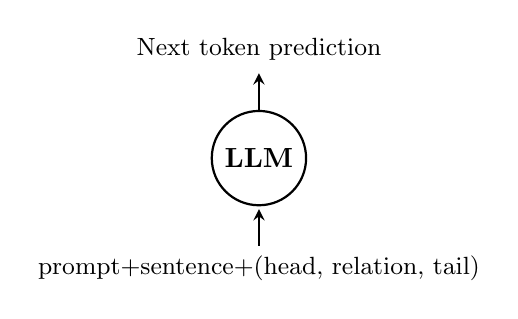
\begin{tikzpicture}[->, >=stealth, shorten >=1pt, auto, thick, main node/.style={circle, draw, font=\small}]

  % Define nodes
  \node[main node, rectangle,opacity=0,text opacity=1] (s0) {prompt+sentence+(head, relation, tail)};
  \node[main node] (s1) [above=.5cm of s0] {\normalsize\textbf{LLM}};
  \node[main node, rectangle,opacity=0,text opacity=1] (s2) [above=.5cm of s1] {Next token prediction};

  % Define edges with labels (including new s1->s2 edge)
  \path[->] 
    (s0) edge node {} (s1)
    (s1) edge node {} (s2);
\end{tikzpicture}
\label{fig:inference_graph}
\end{figure}
\column{.45\textwidth}
\textbf{Evaluation}
\begin{figure}[H]
\centering
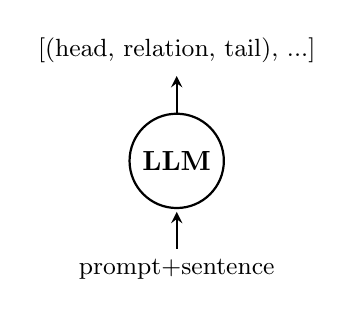
\begin{tikzpicture}[->, >=stealth, shorten >=1pt, auto, thick, main node/.style={circle, draw, font=\small}]

  % Define nodes
  \node[main node,rectangle,opacity=0,text opacity=1] (s0) {prompt+sentence};
  \node[main node] (s1) [above=.5cm of s0] {\normalsize\textbf{LLM}};
  \node[main node,rectangle,opacity=0,text opacity=1] (s2) [above=.5cm of s1] {[(head, relation, tail), ...]};

  % Define edges with labels (including new s1->s2 edge)
  \path[->] 
    (s0) edge node {} (s1)
    (s1) edge node {} (s2);
\end{tikzpicture}
\label{fig:finetune_graph}
\end{figure}
\end{columns}
\end{frame}
\begin{frame}[fragile]{Prompt}
\begin{minted}[fontsize=\normalsize]{text}
List of predicates is [...]. What Subject-Predicate-Object triples are included in the following sentence?
\end{minted}
\end{frame}
\begin{frame}[fragile]{Dataset Transformations: Train sample}
\begin{columns}[c]
\column{.45\textwidth}
\textbf{Sentence-Triples Columns:}
\begin{minted}[fontsize=\tiny]{python}
{
    'sentence': 'Book by arthur laurents, suggested by the memoirs of gypsy rose lee; music by jule styne; lyrics by stephen sondheim; directed by mr. laurents; choreography by jerome robbins, reproduced by bonnie walker; music director-arranger, patrick vaccariello; sets by james youmans; costumes by martin pakledinaz; lighting by howell binkley; sound by dan moses schreier; production stage manager, craig jacobs; orchestrations by sid ramin and robert ginzler; dance arrangements by john kander; music coordinator, seymour red press.', 
    'labels': "[('Jerome Robbins', 'NA', 'James Youmans')]"
}
\end{minted}
\column{.45\textwidth}
\textbf{ChatML:}
\begin{minted}[fontsize=\tiny]{python}
{
    'messages': "<|user|>\nList of predicates is [...].  What Subject-Predicate-Object triples are included in the following sentence?\n Sentence: Book by arthur laurents, suggested by the memoirs of gypsy rose lee; music by jule styne; lyrics by stephen sondheim; directed by mr. laurents; choreography by jerome robbins, reproduced by bonnie walker; music director-arranger, patrick vaccariello; sets by james youmans; costumes by martin pakledinaz; lighting by howell binkley; sound by dan moses schreier; production stage manager, craig jacobs; orchestrations by sid ramin and robert ginzler; dance arrangements by john kander; music coordinator, seymour red press.<|end|>\n<|assistant|>\n[('Jerome Robbins', 'NA', 'James Youmans')]<|end|>\n<|endoftext|>"
}
\end{minted}
\end{columns}
\end{frame}
\begin{frame}[fragile]{Dataset Transformations: Validation/Test Sample}
\begin{columns}[c]
\column{.45\textwidth}
\textbf{Sentence-Triples Columns:}
\begin{minted}[fontsize=\tiny]{python}
{
    'sentence': 'The spokesman of the nigeria police force emmanuel ojukwu told reporters in abuja that 162 of the suspects were already being prosecuted.', 
    'labels': "[('Nigeria Police Force', 'NA', '162')]"
}
\end{minted}
\column{.45\textwidth}
\textbf{ChatML:}
\begin{minted}[fontsize=\tiny]{python}
{
    'labels': "[('Nigeria Police Force', 'NA', '162')]", 
    'messages': "<|user|>\nList of predicates is [...].  What Subject-Predicate-Object triples are included in the following sentence?\n Sentence: The spokesman of the nigeria police force emmanuel ojukwu told reporters in abuja that 162 of the suspects were already being prosecuted.<|end|>\n<|assistant|>\n"
}
\end{minted}
\end{columns}
\end{frame}

\begin{frame}[fragile]{Model and Training: Phi-3-mini}
\begin{itemize}
\item Costly requests to web APIs
\item Availability of resources
\item Performance per number of parameters
\end{itemize}
\begin{minted}[fontsize=\footnotesize]{python}
# LoRA rank r=16
print_info_params(
    model,
    size_type_to_print=("GB", "MB"),
    print_trainable="a",
    calc_param_counts = False,
    calc_grad_counts = False,
)
\end{minted}
\begin{minted}[fontsize=\footnotesize]{text}
>>> all params: 2035321856 || all size: 2.5 GB || trainable params: 26181632 || trainable size: 99.8 MB || trainable%: 1.3 || nontrainable params: 2009140224 || nontrainable size: 2.4 GB || nontrainable%: 98.7
\end{minted}
\end{frame}
\begin{frame}[fragile]{Model and Training: Q-LoRA}
\begin{minted}[fontsize=\normalsize]{python}
bnb_config = BitsAndBytesConfig(
    load_in_4bit=True,
    bnb_4bit_quant_type="nf4",
    bnb_4bit_use_double_quant=True,
    bnb_4bit_compute_dtype=compute_dtype, 
    max_seq_length=4096
)
model = AutoModelForCausalLM.from_pretrained(
    "microsoft/Phi-3-mini-4k-instruct",
    torch_dtype=compute_dtype,
    trust_remote_code=True,
    device_map="cuda",
    attn_implementation='eager',
    quantization_config=bnb_config,
)
\end{minted}
\end{frame}
\begin{frame}[fragile]{Model and Training: Gradient Checkpointing}
\begin{minted}[fontsize=\normalsize]{python}
model = prepare_model_for_kbit_training(
    model,
    use_gradient_checkpointing=True,
    gradient_checkpointing_kwargs={"use_reentrant": True}
)
\end{minted}
\end{frame}
\begin{frame}[fragile]{Model and Training: Gradient accumulation}
\begin{minted}[fontsize=\normalsize]{python}
...
if (self.batch_step + 1) % self.gradient_accumulation_steps == 0:
    torch.autograd.backward(loss)
    self.optimizer.step()
    self.scheduler.step()
    self.optimizer.zero_grad()
...
\end{minted}
\end{frame}
\begin{frame}[fragile]{Cross Entropy}
\begin{minted}[fontsize=\normalsize]{python}
def loss_function(self, batch):
    ...
    metric_adv = 1 # N
    labels_index = labels.view(*labels.shape, 1) # (N, L, 1)
    lpa = torch.gather(log_probs, index=labels_index, dim=-1).squeeze(-1) # (N, L)
    ...
\end{minted}
\end{frame}
\begin{frame}[fragile]{Self-Critical Sequence Training}
\begin{block}{REINFORCE algorithm}
1) Predict the reward $G_t$
\end{block}
\begin{minted}[fontsize=\tiny]{python}
def loss_function(self, batch):
    ...
    actions_amax = logits.argmax(dim=-1) # (N, L)
    scale_amax = calc_scale(actions_amax, labels) if self.baseline else 0 # N
    scale_sample = None
    if self.num_samples > 0:
    probs = F.softmax(logits, dim=-1) # (N, L, S)
    probs_view_2d = probs.view(-1, logits.shape[-1]) # (N*L, S)

    actions_sample_2d = torch.multinomial(probs_view_2d, self.num_samples, replacement=True) # (N*L, R)
    actions_sample_2d_T = actions_sample_2d.T # (R, N*L)
    actions_sample = actions_sample_2d_T.reshape(-1, labels.shape[-1]) # (R*N, L)

    labels_sample = labels.expand(self.num_samples, *labels.shape).reshape(-1, labels.shape[-1]) # (R*N, L)
    scale_sample = calc_scale(actions_sample, labels_sample).view(self.num_samples,-1) # (R, N)
    # -(Q - b)
    metric_adv = scale_amax - scale_sample # (R,N)
    ...
\end{minted}
\end{frame}
\begin{frame}[fragile]{Self-Critical Sequence Training}
    \begin{block}{REINFORCE algorithm}
        2) Perform a gradient update $\theta \leftarrow \theta + \alpha \gamma^t G_t \nabla_\theta \ln \pi_\theta(A_t \vert S_t)$\ \cite{weng_policy_2018}
    \end{block}
\begin{minted}[fontsize=\normalsize]{python}
def loss_function(self, batch):
    ...
    actions_sample_index = actions_sample.view(self.num_samples, *labels.shape,1) # (R, N, L, 1)
    log_probs_expanded = log_probs.expand(self.num_samples, *log_probs.shape) # (R, N, L, S)
    lpa = torch.gather(log_probs_expanded, index=actions_sample_index, dim=-1).squeeze(-1) # (R, N, L)
    ...
\end{minted}
\end{frame}
\begin{frame}[fragile]{Smoothed Return}
\begin{minted}[fontsize=\normalsize]{python}
def loss_function(self, batch):
    ...
    lpa.masked_fill_(padding_mask, 0.0) # (R, N, L) or (N, L)
    lpa_len_1 = len(lpa.shape)-1
    lpa_permuted = lpa.permute(lpa_len_1, *range(lpa_len_1)) # (L, R, N) or (L, N)
    loss = metric_adv * lpa_permuted # (L, R, N) or (L, N)
    loss = loss.sum() / num_active_elements
    return (1 - self.label_smoothing_factor) * loss + self.label_smoothing_factor * smoothed_loss
\end{minted}
\end{frame}
\begin{frame}[fragile]{Self-Critical Sequence Training: Rewards}
\begin{minted}[fontsize=\scriptsize]{python}
def loss_function(self, batch):
    ...
    def calc_scale(candidates, references):
      candidates_detokenized = self.tokenizer.batch_decode(
        candidates,
        skip_special_tokens=True,
        clean_up_tokenization_spaces=True,
      )
      references_detokenized = self.tokenizer.batch_decode(
        references,
        skip_special_tokens=True,
        clean_up_tokenization_spaces=True,
      )
      def ret_metric(res):
        return res if self.train_metric_key==None else res[self.train_metric_key]
      if self.multiple:
        res = [ret_metric(self.train_metric([c], [references_detokenized])) for c in candidates_detokenized]
      else:
        res = [ret_metric(self.train_metric([c], [[r]])) for c, r in zip(candidates_detokenized, references_detokenized)]
      return torch.tensor(res).to(self.model.device)
      ...
\end{minted}
\end{frame}
\begin{frame}[fragile]{Evaluation}
\begin{minted}[fontsize=\footnotesize]{python}
class MicroF1(CustomMetric):
    ...
    def forward(self, raw_text_preds, raw_text_true):
        raw_text_preds = raw_text_preds.strip("` \n")
        if raw_text_preds.startswith("python"):
            raw_text_preds = self.fix(raw_text_preds)
        preds_triples = eval(raw_text_preds)
        true_triples = eval(raw_text_true)
        preds_triples_set = set(preds_triples)
        true_triples_set = set(true_triples)
        true_positives = preds_triples_set & true_triples_set # intersection set
        lentp = len(true_positives)
        self.tps += lentp # add intersection cardinal
        self.total += (len(preds_triples) + len(true_triples) - lentp) # add union cardinal
        return raw_text_preds, raw_text_truedef ret(self):
        if self.total == 0:
            return 0
        return self.tps / self.totaldef fix(self, raw_text_preds):
        return raw_text_preds[raw_text_preds.index("["):]
\end{minted}
\end{frame}
\begin{frame}[fragile]{Hyperparameter Tuning}
\begin{minted}[fontsize=\normalsize]{python}
def objective(trial):
  train_metric_key = trial.suggest_categorical("train_metric_key", [None, 'rouge1_fmeasure', 'rouge2_fmeasure', 'rougeL_fmeasure', 'rougeLsum_fmeasure'])
  if train_metric_key == None:
    num_samples = trial.suggest_int("num_samples", 0, 4)
    if num_samples == 0:
      train_metric = None
    else:
      train_metric = BLEUScore(n_gram=4, smooth=True)
  else:
    num_samples = trial.suggest_int("num_samples", 1, 4)
    train_metric = ROUGEScore(use_stemmer=True, accumulate='avg')
    ...
\end{minted}
\end{frame}
\begin{frame}[fragile]{Hyperparameter Tuning}
\begin{minted}[fontsize=\tiny]{python}
def objective(trial):   
    ...
    beta1 = trial.suggest_float("beta1", 0.5, 1-EPSILON, log=True)
    beta2 = trial.suggest_float("beta2", beta1, 1-EPSILON, log=True)
    params = {
        # LOSS KWARGS
        "label_smoothing_factor": trial.suggest_float("label_smoothing_factor", EPSILON, 1, log=True),#
        "train_metric": train_metric,#
        "train_metric_key": train_metric_key,#
        "num_samples": num_samples,#
        "multiple": trial.suggest_categorical("multiple", [True, False]),#
        # GEN KWARGS
        "do_sample": trial.suggest_categorical("do_sample", [True, False]),#
        "num_beams": trial.suggest_int("num_samples", 1, 4),
        "temperature": trial.suggest_float("temperature", EPSILON, 2, log=True),
        "top_p": trial.suggest_float("top_p_1", EPSILON, 1, log=True),
        # MODEL KWARGS
        "lora_r": trial.suggest_int("lora_r", 1, 64),#
        "lora_dropout": trial.suggest_float("lora_dropout", EPSILON, 1, log=True),#
        # OPTIM KWARGS
        "optim_arg": OptimArg(
        name="AdamW",
            args={
                "lr": trial.suggest_float("weight_decay", 1e-20, 1e-1, log=True), #1e-8
                "betas": (beta1, beta2), #(0.9, 0.999)
                "weight_decay": trial.suggest_float("weight_decay", 1e-4, 1e-1, log=True), #1e-2
            },
        )#,
    }
    ...
\end{minted}
\end{frame}
\subsection{Results}
\begin{frame}{Results}
\end{frame}
\section{Self-Reflection and Future Directions}
\begin{frame}{Self-Reflection and Future Directions}
\begin{itemize}
    \item Implementation of Trainer API
    \begin{itemize}
        \item External API
        \item PyTorch Lightning
    \end{itemize}
    \item More constraints (e.g A number of ontological features in input)
    \item Model+knowledge base
    \item Novel models (e.g Phi-4, DeepSeek)
\end{itemize}
\end{frame}

\begin{frame}{References}
    \footnotesize
    \bibliography{refs.bib}
    \bibliographystyle{IEEEtran}
\end{frame}

%------------------------------------------------

\begin{frame}
    \Huge{\centerline{\textbf{Thank you for listening}}}
\end{frame}

%----------------------------------------------------------------------------------------

\end{document}